\tikzstyle{startstop} = [rectangle, rounded corners, minimum width=3cm, minimum height=1cm,text centered, text width=3cm, draw=black, fill=red!30]
\tikzstyle{process} = [rectangle, minimum width=3cm, minimum height=1cm, text centered, text width=2.5cm, draw=black, fill=orange!30]
\tikzstyle{decision} = [rectangle, minimum width=3cm, minimum height=1cm, text centered, text width=2.5cm, draw=black, fill=green!30]
\tikzstyle{arrow} = [thick,->,>=stealth]
    
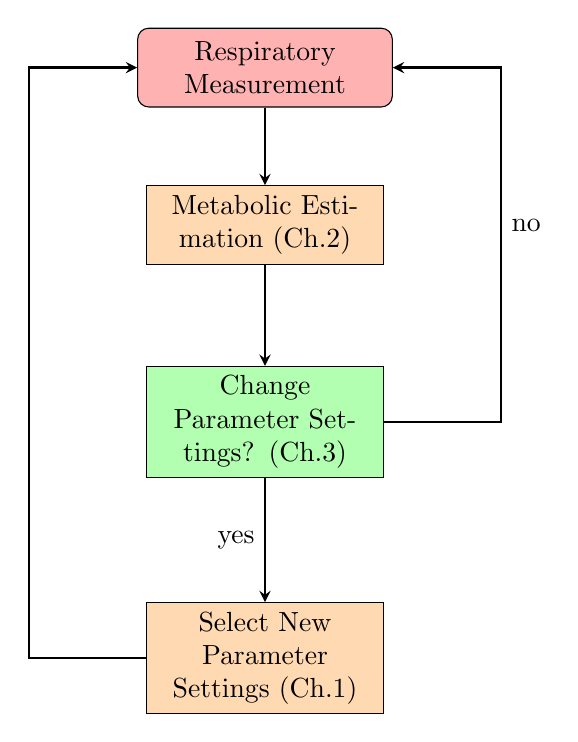
\begin{tikzpicture}[node distance=2cm]

\node (measurement) [startstop] {Respiratory Measurement};
\node (estimator) [process, below of=measurement] {Metabolic Estimation (Ch.2)};
\node (stopping) [decision, below of=estimator, yshift=-0.5cm] {Change Parameter Settings? (Ch.3)};
\node (bayesopt) [process, below of=stopping, yshift=-1cm] {Select New Parameter Settings (Ch.1)};

\draw [arrow] (measurement) -- (estimator);
\draw [arrow] (estimator) -- (stopping);
\draw [arrow] (stopping) --++ (3cm,0cm) |- node[anchor=west, yshift=-2cm] {no} (measurement);
\draw [arrow] (stopping) -- node[anchor=east] {yes} (bayesopt);
\draw [arrow] (bayesopt) --++ (-3cm,0cm) |- (measurement);


\end{tikzpicture}